%%%%%%%%%%%%%%%%%%%%%%%%%%%%%%%%%%%%%%%%%%%%%%%%%%%%%%%%%%%%%%%%%%%%%%%%
%                                                                      %
%     File: Thesis_Evaluation.tex                                         %
%     Tex Master: Thesis.tex                                           %
%                                                                      %
%     Author: Andre C. Marta                                           %
%     Last modified :  2 Jul 2015                                      %
%                                                                      %
%%%%%%%%%%%%%%%%%%%%%%%%%%%%%%%%%%%%%%%%%%%%%%%%%%%%%%%%%%%%%%%%%%%%%%%%

\chapter{Evaluation}
\label{chapter:evaluation}

%%%%%%%%%%%%%%%%%%%%%%%%%%%%%%%%%%%%%%%%%%%%%%%%%%%%%%%%%%%%%%%%%%%%%%%%
\section{Test Methodology}
\label{section:test-methodology}

We implemented our CRSH algorithm in OpenGL/C++ and CUDA/C++ then compared it with our implementation of RAH \cite{Roger07} over the same architecture. We map our algorithm onto the GPU, parallelizing it there fully. We achieve this mainly by the use of parallel primitives, like prefix sums \cite{Blelloch90}. We used the CUB \cite{Merrill09}  \cite{Merrill11} library to perform parallel radix sorts and prefix sums.

We measure the amount of intersections, including misses and hits, to evaluate ray hierarchy algorithms proficiency at reducing the amount of ray-primitive intersection tests required to render an image. All scenes were rendered at $512\times512$ resolution.

The test information was collected using a NVIDIA GeForce GTX TITAN GPU with 6 GB of RAM. Our algorithm is completely executed on the GPU (including hierarchy construction and traversal) so the CPU has no impact on the test results.

%%%%%%%%%%%%%%%%%%%%%%%%%%%%%%%%%%%%%%%%%%%%%%%%%%%%%%%%%%%%%%%%%%%%%%%%
\section{Test Scenes}
\label{section:test-scenes}

We used three different scenes, \textsc{Office}, \textsc{Cornell} and \textsc{Sponza}.

The \textsc{Office} scene (36K triangles) is representative of interior design applications. It is divided into several submeshes therefore it adapts very well to our bounding volume scheme. For this scene the emphasis was on testing shadow rays. 

We selected \textsc{Cornell} (790 triangles). as it is representative of highly reflective scenes. It consists an object surrounded by six mirrors. On this scene we focused on testing reflection rays although it also features shadow rays in it.

\textsc{Sponza} (66K triangles), much like \textsc{Office}, is representative of architectural scenes. For this scene the emphasis was also on testing shadow rays but for scenes that do not conform with our bounding volume scheme. This scene does not adapt well to our scheme as is not divided into submeshes. 

%%%%%%%%%%%%%%%%%%%%%%%%%%%%%%%%%%%%%%%%%%%%%%%%%%%%%%%%%%%%%%%%%%%%%%%%
\section{Test Results and Discussion}
\label{section:test-results-and-discussion}

We hypothesised that our more coherent RSH hierarchy needs to compute fewer intersection results to render a scene. We expect more expressive results for shadow rays. As shadow rays have low divergence the sorting step should create a more coherent RSH than for reflection rays. In addition our hierarchy should also be more coherent with reflection rays than one based on the RAH algorithm due to the hashing we use. However by the very nature of reflection rays they will never be as coherent as shadow rays resulting in a lower quality hierarchy.

\begin{table}[!htb]
\begin{center}
\fontencoding{T1}
\fontseries{m}
\fontshape{sc}
\fontsize{7}{9}
\selectfont
\begin{tabular}{l|rrr}
    \multicolumn{1}{c}{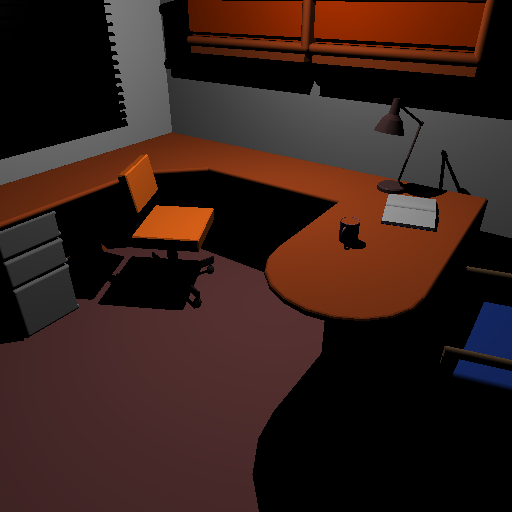
\includegraphics[width=1.5cm]{Images/Office_Preview}} & & \\
    \multicolumn{1}{c|}{\textsc{Office}} & \textsc{Level 1} & \textsc{Level 2} & \textsc{Level 3}\\
    \hline
    \emph{RAH Algorithm} & & \\
    \hline
    \quad \# Sh Intersections  & 17863536	 & 131228368    & 202134400  \\
    \quad Sh Misses            & 1459990	 & 105961568    & 186536226	 \\
    \quad Sh Hits              & 16403546	 & 25266800	    & 15598174	 \\

    & & \\

    \hline
    \emph{Our Algorithm} & & \\
    \hline
    \quad \# Sh Intersections   & 4108164	     & 31863128	    & 75095808	 \\
    \quad Sh Misses    & 125148		 & 21144630	    & 57127535	 \\
    \quad Sh Hits & 3983016		 & 10718498	    & 17968273	 \\
\end{tabular}
\end{center}
\caption{\label{table:office-results}
\textsc{Office} rendering performance (251546 shadow rays).}
\end{table}

Our initial expectations for Office were to get a much lower number of intersection tests with our algorithm than with RAH. The scene is a good fit to our bounding volume scheme and our highly coherent shadow ray hierarchy. Results confirm (see Table~\ref{table:office-results}) our initial expectations: we compute 46\% less intersections than RAH on this scene. 97,21\% less than a brute force approach.

\begin{table}[!htb]
\begin{center}
\fontencoding{T1}
\fontseries{m}
\fontshape{sc}
\fontsize{7}{9}
\selectfont
\begin{tabular}{l|rrr}
    \multicolumn{1}{c}{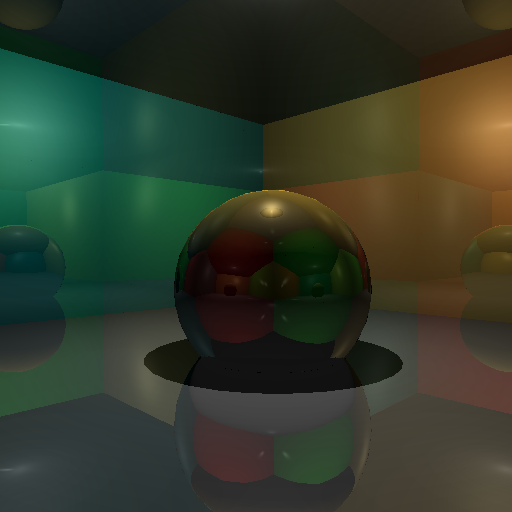
\includegraphics[width=1.5cm]{Images/Cornell_Preview}} & & \\
    \multicolumn{1}{c|}{\textsc{Cornell}} & \textsc{Level 1} & \textsc{Level 2} & \textsc{Level 3}\\
    \hline
    \emph{RAH Algorithm} & & \\
    \hline
    \quad \# Sh Intersections   & 805752	 & 5556560		& 10814328	 \\
    \quad Sh Misses             & 111182	 & 4204769	    & 9227709	 \\
    \quad Sh Hits               & 694570	 & 1351791		& 1586619	 \\
    & & \\
    \quad \# Re Intersections   & 2285568	 & 18143152	    & 54373424	 \\
    \quad Re Misses             & 17674		 & 11346474	    & 48340898	 \\
    \quad Re Hits               & 2267894	 & 6796678	    & 6032526    \\

    & & \\

    \hline
    \emph{Our Algorithm} & & \\
    \hline
    \quad \# Sh Intersections   & 370152		 & 1768864	    & 4130048	 \\
    \quad Sh Misses             & 149044		 & 1252608		& 2891984	 \\
    \quad Sh Hits               & 221108		 & 516256	    & 1238064	 \\
    & & \\
    \quad \# Re Intersections   & 1787712	     & 12600640	    & 30460504	 \\
    \quad Re Misses             & 212632		 & 8793077	    & 24908902   \\
    \quad Re Hits               & 1575080		 & 3807563	    & 5551602	 \\
\end{tabular}
\end{center}
\caption{\label{table:cornell-results}
\textsc{Cornell} rendering performance (184717 shadow \& 524288 reflection rays).}
\end{table}

For the Cornell scene we focused primarily on the reflection rays which are much more incoherent than shadow rays so we expected results to be less positive than with the Office scene. We compute 32\% less intersections overall (shadow and reflection rays combined) than the RAH algorithm and 93,15\% less than the brute force approach (see Table~\ref{table:cornell-results}).

\begin{table}[!htb]
\begin{center}
\fontencoding{T1}
\fontseries{m}
\fontshape{sc}
\fontsize{7}{9}
\selectfont
\begin{tabular}{l|rrr}
    \multicolumn{1}{c}{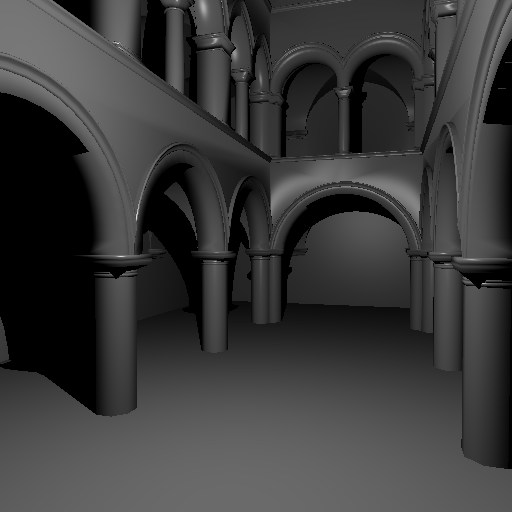
\includegraphics[width=1.5cm]{Images/Sponza_Preview}} & & \\
    \multicolumn{1}{c|}{\textsc{Sponza}} & \textsc{Level 1} & \textsc{Level 2} & \textsc{Level 3}\\
    \hline
    \emph{RAH Algorithm} & & \\
    \hline
    \quad \# Sh Intersections  & 33357900	 & 200061944    & 261267720  \\
    \quad Sh Misses            & 6487857	 & 182303479    & 248568705	 \\
    \quad Sh Hits              & 26870043	 & 17758465	    & 12699015	 \\

    & & \\

    \hline
    \emph{Our Algorithm} & & \\
    \hline    
    \quad \# Sh Intersections  & 33357900	& 23359968	& 61887672	 \\
    \quad Sh Misses            & 30437904	& 15624009	& 53120871	 \\
    \quad Sh Hits              & 2919996	& 7735959	& 8766801	 \\
\end{tabular}
\end{center}
\caption{\label{table:sponza-results}
\textsc{Sponza} rendering performance (256713 shadow rays).}
\end{table}

\begin{table*}[!htb]
\begin{center}
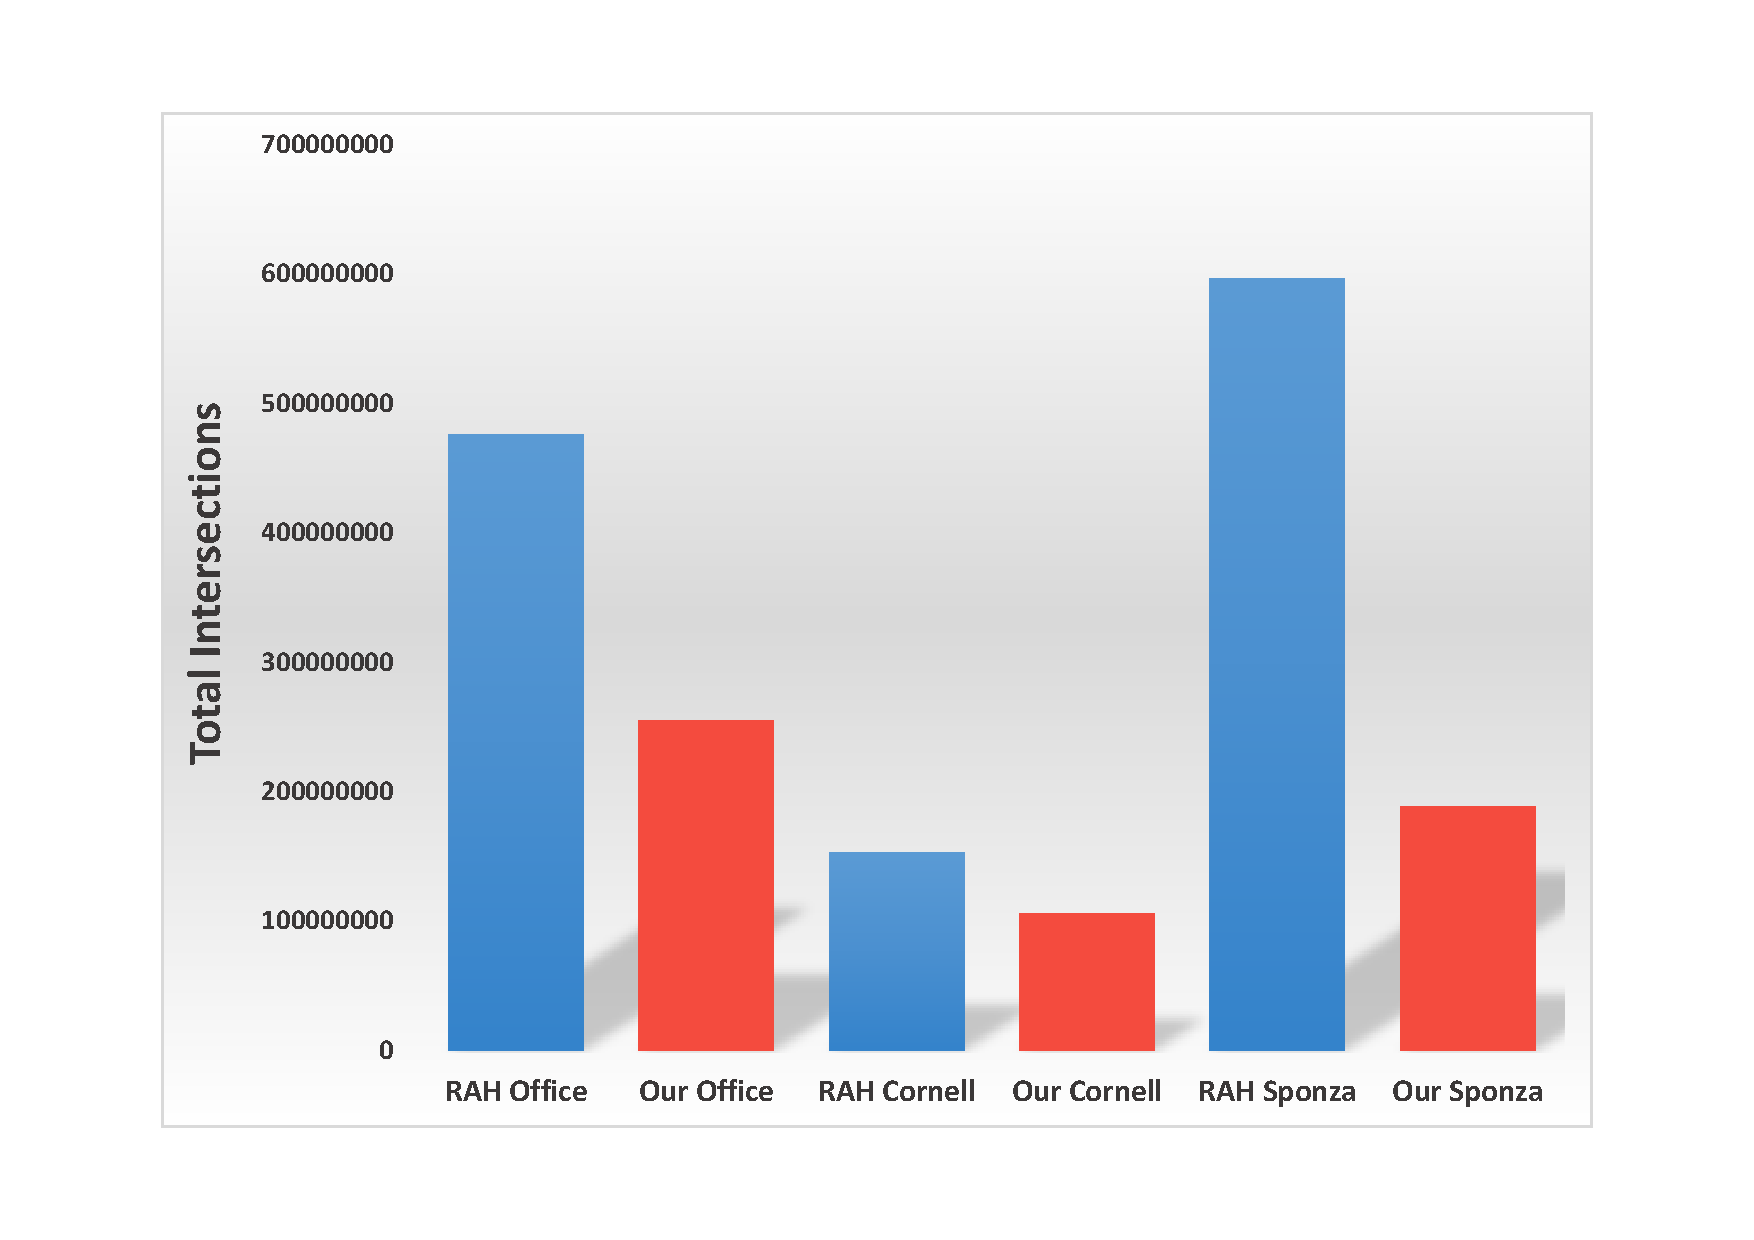
\includegraphics[width=0.45\textwidth]{Images/Result_Chart}
\vskip 1em
\fontencoding{T1}
\fontseries{m}
\fontshape{sc}
\fontsize{7}{9}
\selectfont
\begin{tabular}{l|rrrrrr}
& \multicolumn{2}{c}{\textsc{Office}} & \multicolumn{2}{c}{\textsc{Cornell}} & \multicolumn{2}{c}{\textsc{Sponza}} \\
\textsc{Algorithm} & \textsc{Total \# isect} & \textsc{Relative \%} & \textsc{Total \# isect} & \textsc{Relative \%} & \textsc{Total \# isect} & \textsc{Relative \%} \\
    \hline
    \emph{Brute Force}     & 9133132168        & 100\% & 153995886          & 100\% & 17058578850 & 100\% \\
    \emph{RAH Algorithm}   & 476011696         & 5.12\% & 152931944			& 9.93\% & 596279684 & 3.50\% \\
    \emph{Our Algorithm}   & \textbf{254813284} & \textbf{2.79\%} & \textbf{105435248} & \textbf{6.85\%} & \textbf{188739948} & \textbf{1.11\%} \\
\end{tabular}
\end{center}
\caption{\label{tab:results}
\small\textsc{Office} (251546 shadow rays), \textsc{Cornell} (184717 shadow \& 524288 reflection rays), \textsc{Sponza} (256713 shadow rays)  rendering performance.}
\end{table*}

The final scene, Sponza, is a whole mesh. We did not employ object subdivision in this scene. Hence we expected worse results than with Office since we would only get the benefit of the shadow ray hierarchy and none from the bounding volume scheme. To our surprise, however, our CRSH algorithm actually manages to outperform RAH in Sponza by a bigger margin than in the Office scene.

We compute 69\% less intersection tests than RAH and 98,89\% than the brute force approach. These results are due to the number of potential hits culled in the first level of the hierarchy (see Table~\ref{table:sponza-results}). Since our CRSH is more coherent, our algorithm culls 91\% of those hits at the first level while RAH only culls 19\%.